%%
%% Beuth Hochschule für Technik --  
%%
%% Kapitel 3 -
%%
%%	


%%%%%%%%%%%%%%%%%%%%%%%%%%
%% bild einfügen:

%\begin{figure}[h]
%	\begin{center}
%		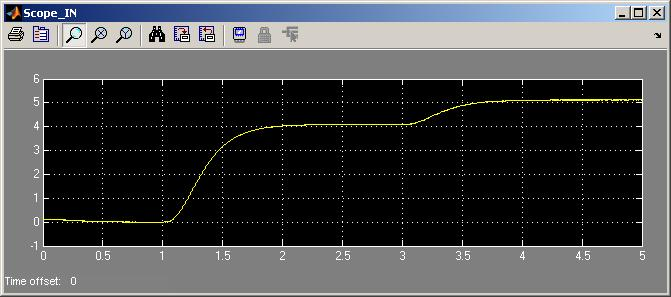
\includegraphics[scale=0.5]{sprungantwort.jpg}
%		\caption{bildbeschreibung - titel}
%       \label{für referenzen}
%	\end{center} 
%\end{figure}


%wenn du auf das bild refenzieren willst schreibst du \ref{...} wo ... = der inhalt von \label{•}

% sys_id = sys\_id ...... für latex _ = \_

%namen von dateien und tools bitte immer italic --> \textit{.....}

% mathematische werte zB 0,5V schreibst du so: $0,5V$

\newpage
[Perkowski]
\section{Messtechnische Identifikation des Steuerverhaltens der Strecke}


\subsection{Dynamisches Verhalten}

Zur Ermittlung des dynamischen Verhaltens wird eine Messung durchgeführt, in der die Strecke mit einem Sprung an der Stellgröße erregt wird. Wir wissen bereits, dass der Arbeitspunkt bei $50 bar$ beträgt, daher können wir das System in der Nähe des Arbeitspuntes (mit einem Sprung von $4V$ auf $5V$) erregen.

\begin{figure}[h]
	\begin{center}
		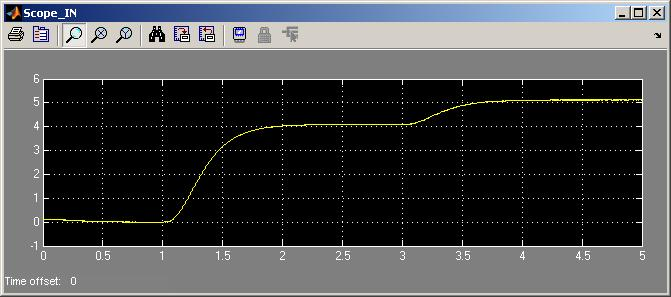
\includegraphics[scale=0.5]{sprungantwort.jpg}
		\caption{Sprungantwort - dynamische Kennlinie}
       \label{dynsprant}
	\end{center} 
\end{figure}

\subsection{Identifikation der Strecke}
Mit Hilfe des Tools \textit{sis\_id.m} können wir die Strecke identifizieren. Dafür müssen die Vektoren \textit{ySystem} (Sprungantwort), \textit{uerr} (Sprung) und \textit{t} (Zeitachse) im Workspace bekannt sein. Im Tool \textit{sis\_id.m} muss eine Vorauswahl der Übertragungsglieder erfolgen. Da die Sprungantwort am Anfang eine Verzögerung hat, handelt es sich mindestens um ein PT2-Glied. Nach der Berechnung und Ausprobieren von sys\_id ist im Abb. zu sehen, dass am Ende die Strecke aus einem System besteht, das in Reihe PT1, PT2 und PT3 geschaltet ist. Die Parameter der Übertragungsfunktion in V-Normalform können unter im Feld abgelesen werden. Die Übertragungsfunktion kann mit Button \textit{"Model speichern"} in der Form von Polynom im Workspace abgespeichert werden.

\begin{figure}[h]
	\begin{center}
		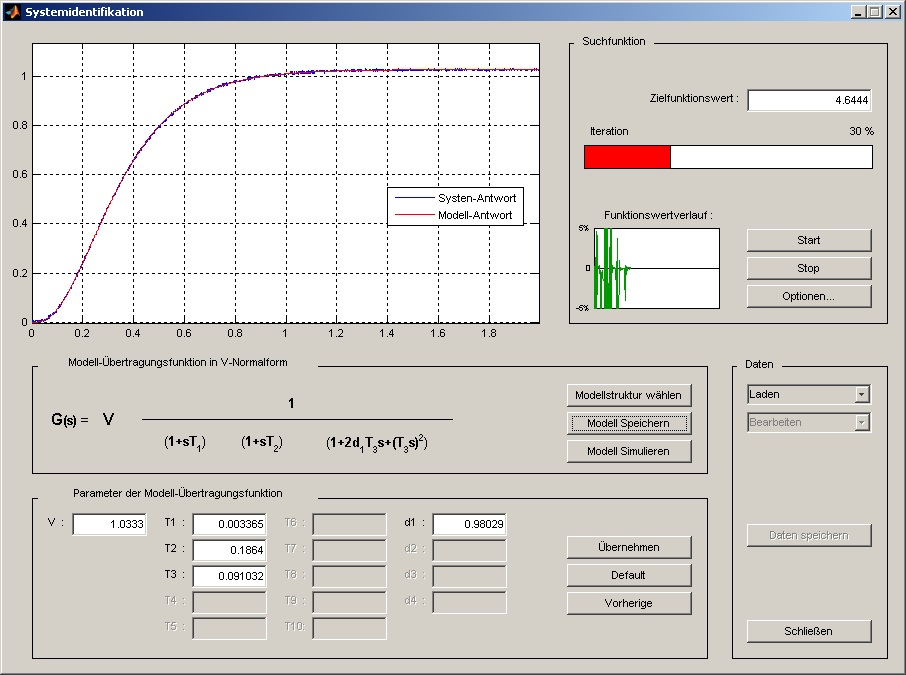
\includegraphics[scale=0.5]{sysid.jpg}
		\caption{Tool \textit{sis\_id} für Identifikation der Strecke}
       \label{pic_sis_id}
	\end{center} 
\end{figure}

Die ermittelte Übertragungsfunktion aus dem Tool \textit{sis\_id}: 

\begin{center}
$ G(s) = \dfrac{1,03}{(1 + 0,003365s) * (1 + 0,1864s) * (1 + 2*0,98029s + (0,091032s)^{2}) }$
\end{center}

Ausmultiplizierte Übertragungsfunktion für Polkompensation:

\begin{center}
$ G(s) =  \dfrac{1,03}{0,000005s^{4} + 0,0017s^{3	} + 0,043s^{2} + 0,368s + 1 } $
\end{center}
